\documentclass[xcolor=dvipsnames,10pt]{beamer}

\mode<presentation> {\usetheme{Singapore}}
\usepackage{pgfpages}

%\setbeamercovered{transparent} 
\usepackage[english]{babel}
\usepackage[latin1]{inputenc}
\usepackage{times,amsfonts}
\usepackage[T1]{fontenc}
\setlength{\parskip}{\baselineskip}
% Or whatever. Note that the encoding and the font should match. If T1
% does not look nice, try deleting the line with the fontenc.

%\usecolortheme{sidebartab}
\setbeamertemplate{itemize item}[triangle]



\usepackage{calc}
\usepackage{environ}
\newcommand{\halfmargin}{0.0001\paperwidth}


\RequirePackage{booktabs,colortbl,ulem}

\usepackage{animate}
\RequirePackage{booktabs,colortbl,gensymb}
\setlength{\parskip}{\baselineskip}

\usepackage{calc}
\usepackage{environ}

% \newcommand{\halfmargin}{0.0001\paperwidth}


\NewEnviron{wideframe}[1][]{%
\begin{frame}{#1}
\makebox[\textwidth][c]{
\begin{minipage}{\dimexpr\paperwidth-\halfmargin-\halfmargin\relax}
\BODY
\end{minipage}}
\end{frame}
}


\DeclareMathOperator{\stdev}{stdev}
\DeclareMathOperator{\var}{var}
\DeclareMathOperator{\cov}{cov}
\DeclareMathOperator{\corr}{corr}
\DeclareMathOperator{\prob}{prob}
\DeclareMathOperator{\n}{n}
\DeclareMathOperator{\N}{N}
\DeclareMathOperator{\Cov}{Cov}

\newcommand{\hlf}{\frac{1}{2}}
\newcommand{\bi}{\begin{itemize}}
\newcommand{\ei}{\end{itemize}}
\newcommand{\im}{\item}
\newcommand{\D}{\mathrm{d}}
\newcommand{\E}{\mathrm{e}}
\newcommand{\mye}{\ensuremath{\mathsf{E}}}
\newcommand{\myreal}{\ensuremath{\mathbb{R}}}
\newcommand{\bq}{\begin{equation}}
\newcommand{\eq}{\end{equation}}
\newcommand{\eqdef}{\;\buildrel \text{d{}ef}\over = \;}
\newcommand{\xstar}{\buildrel *\over X}
\newcommand{\pmax}{p^{\text{max}}}
\newcommand{\qmax}{q^{\text{max}}}
\newcommand{\bfr}{\begin{frame}}
\newcommand{\bfrp}{\begin{frame}[plain]}
\newcommand{\efr}{\end{frame}}
\newcommand{\F}{\mathcal{F}}
\newcommand{\FF}{\mathbb{F}}
\newcommand{\ve}{\varepsilon}
\newcommand{\lh}{\hat{\lambda}}
\definecolor{mycolor}{gray}{0.8}
\definecolor{mymaincolor}{rgb}{0.6862745098039216,0.9333333333333333,0.9333333333333333}
\newcommand{\alr}[1]{\textcolor{blue}{#1}}
\definecolor{LightCyan}{rgb}{0.88,1,1}
\newcommand{\yel}{\cellcolor{yellow}}
\newcommand{\blue}{\cellcolor{SkyBlue}}
\newcommand{\gr}{\cellcolor{SpringGreen}}
\newcommand{\pink}{\cellcolor{pink}}
\newcommand{\apr}{\cellcolor{Apricot}}
\newcommand{\tve}{\tilde{\varepsilon}}
\newcommand{\tw}{\tilde{w}}
\newcommand{\ttth}{\tilde{\theta}}
\newcommand{\te}{\tilde{e}}
\newcommand{\ts}{\tilde{s}}
\newcommand{\tx}{\tilde{x}}
\newcommand{\ty}{\tilde{y}}
\newcommand{\tv}{\tilde{v}}
\newcommand{\tp}{\tilde{p}}
\newcommand{\tF}{\tilde{F}}
\newcommand{\tf}{\tilde{f}}
\newcommand{\tZ}{\tilde{Z}}
\newcommand{\ow}{\overline{w}}
\newcommand{\lb}{\left[}
\newcommand{\rb}{\right]}
\newcommand{\lp}{\left(}
\newcommand{\rp}{\right)}
\newcommand{\tm}{\tilde{m}}
\newcommand{\tc}{\tilde{c}}
\newcommand{\tz}{\tilde{z}}
\newcommand{\str}[1]{\textcolor{blue}{\sout{#1}}}
\newcommand{\tr}{\widetilde{R}}
\newcommand{\tR}{\widetilde{\mathbf{R}}}
\newcommand{\bms}{\begin{multline*}}
\newcommand{\ems}{\end{multline*}}
\newcommand{\bas}{\begin{align*}}
\newcommand{\eas}{\end{align*}}
\newcommand{\qr}{\mathbb{Q}}
\newcommand{\IMAGES}{/home/kerry/Dropbox/Images}
\newcommand{\tX}{\tilde{X}}
\newcommand{\tY}{\tilde{Y}}

\author{\vskip 0.5in \small Kerry Back \\BUSI 521--ECON 505\\ Rice University \\Spring 2022}
%\institute{Rice University\\ Spring 2019}
\date[]





\newcommand{\tu}{\tilde{u}}
\begin{document}
\title{\vskip 0.5in Day 17}
\subtitle{Futures Markets}

\begin{frame}
  \titlepage
\end{frame}

\begin{frame}{Futures Contracts}
    An agreement to transact at a later date.  One party will deliver and be paid.  The other party will accept delivery and will pay.  The contracts have specific maturity dates.
    
    Buyer (long) will accept delivery and will pay.  Seller (short) will deliver and be paid.
    
    Examples: energy (crude oil, natural gas, refined products), metals (gold, silver, \ldots), agricultural, currencies, financials (stock indexes, Treasury bonds, \ldots).
    
    Exchange traded.  Anyone can trade.  Usually buyer will later sell, and seller will later buy, so neither takes or makes delivery.
    
    Some traders are hedging.  Others are speculating.
\end{frame}

\begin{frame}{Margin}
When you buy a contract, you do not pay.  And, when you sell, you do not receive payment.  But both parties have to post collateral (margin) - less than 10\% of the contract value.

Trade is anonymous.  After a trade, the exchange clearinghouse becomes the counterparty to both traders.  

To minimize the risk of anyone defaulting, gains and losses are credited daily, and the contract price is reset to the market price -- called marking to market.
\end{frame}

\begin{frame}{Marking to Market Example}
The CME (Chicago Mercantile Exchange) West Texas Intermediate (WTI) crude oil contract is for 1,000 barrels with delivery in Cushing, Oklahoma.

Suppose you bought 1 CME WTI contract for Dec, 2022 delivery on Jan 2, 2020.  You bought it at \$50.  The contract closed (settled) that day at \$51.
    
You made 1,000 (barrels) $\times$ \$1 per barrel = \$1,000 on Jan 2.  You received that money at the end of the day.  The contract is repriced at \$51, so you are now obliged to pay \$51 when you receive delivery.

Your net price is \$51 - \$1 = \$50.  Your net price will always equal the price at which you bought the contract.
\end{frame}

\begin{frame}[plain]
Consider the seller of the contract at \$50.  Because the price rose \alert{after the sale}, the seller lost money.  She is charged \$1 at the end of the day on Jan. 2.  The contract is repriced to \$51, so she will now be paid \$51 when she delivers.  Her net price is still \$50.

Why this complication?  Suppose the price moves daily in \$1 increments until it hits \$99.  The seller has now paid \$49.  Suppose the next day the price hits \$100 and for some reason (maybe because of money lost elsewhere) the seller declares bankruptcy.  

The clearinghouse has to pay \$1 again to you, because you won again that day.  And, it takes over the seller's contract to deliver at \$100.  Because \$100 is the market price, there is no gain or loss associated with taking over the contract.

What would the gain or loss be if the clearinghouse had to take over a contract to deliver at \$50 when the market price is \$100?
\end{frame}

\begin{frame}{Cash Settled Contracts}
    Some contracts do not have any delivery provisions at all.  They are cash settled at maturity based on market prices.
    
    An example is the CME S\&P 500 e-mini contract.  It is cash settled at \$50 times the index.  (\$50 is the `contract size,' like 1,000 barrels is the WTI contract size).
    
    Suppose you buy the S\&P 500 e-mini contract at a `price' of 4600.  And suppose the index is at 4700 when the contract matures.  You make \$50 $\times (4700-4600) = $ \$5,000.  You will make this in daily increments due to marking to market.
    
    A cash settled contract is just a bet on whether something will go up or down.
    \end{frame}
    
    
\end{frame}

\begin{frame}{Forward Curve}
    At any given time, there are contracts with various maturities trading.  The function \alert{maturity $\mapsto$ price} is called the forward curve.
    
    The entire curve shifts up or down (or twists) on a daily (actually minute-to-minute) basis.
    
    Some forward curves are upward sloping (higher prices at longer maturities) and some are downward sloping and some go up and down.
    
    Upward sloping is called contango.  Downward sloping is called backwardation.
\end{frame}

\begin{frame}{Gold is Always in Contango}
    \begin{center}
        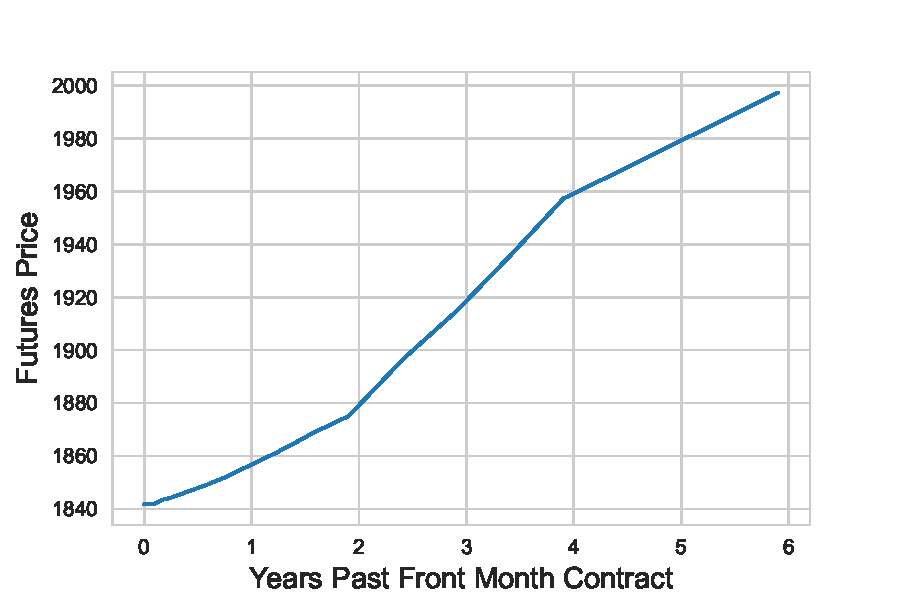
\includegraphics[scale=0.6]{Images/fig_gold.pdf}
    \end{center}
    Gold forward curve on 1-24-2022.  You have to pay a higher price if you want to buy with future settlement.
\end{frame}

\begin{frame}{Why is Gold in Contango?}
    Suppose the gold forward curve is downward sloping.  Suppose you own gold and plan to continue owning gold.  You could sell spot (spot means for `immediate' delivery) and buy futures and pocket the difference in price (plus interest).
    
    Suppose the curve is just flat instead of downward sloping.  You would still sell spot and buy futures.  You can invest the cash from selling spot and earn interest.  You pocket the interest.
    
    But, the gold curve can't be too steep.  If it were, people would buy gold now and sell the futures.
\end{frame}

\begin{frame}{Spot-Futures Parity}

$S=$ spot price, $F=$ futures price, $r=$ continuously compounded interest rate (annual rate), $T=$ time to maturity (in years), $y=$ convenience yield (more later).

$$S \times \E^{(r-y)T} = F$$

So, slope of the log forward curve is $r-y$:

$$\frac{\log F - \log S}{T} = r-y$$
\end{frame}

\begin{frame}{Currency Example}
Consider yen futures.  $S=$ spot price of 1 yen in dollars, $F=$ futures price, $r=$ dollar interest rate, $y=$ yen interest rate.

Synthetic futures: borrow dollars, buy yen, invest yen at yen interest rate. At $T$, you will have yen and pay dollars (to repay the loan).

How many yen to buy?  To have 1 yen in $T$ years, you need to buy and invest $\E^{-yT}$ yen today.  The cost of $\E^{-yT}$ yen is $S\E^{-yT}$.  If you borrow this many dollars, you will owe $S\E^{-yT}\E^{rT}$ dollars in $T$ years.  

The cost of the synthetic futures should be the cost of the actual futures (otherwise, you could arbitrage), so $S\E^{(r-y)T} = F$.
\end{frame}

\begin{frame}{Euro Forward Curve}
    \begin{center}
        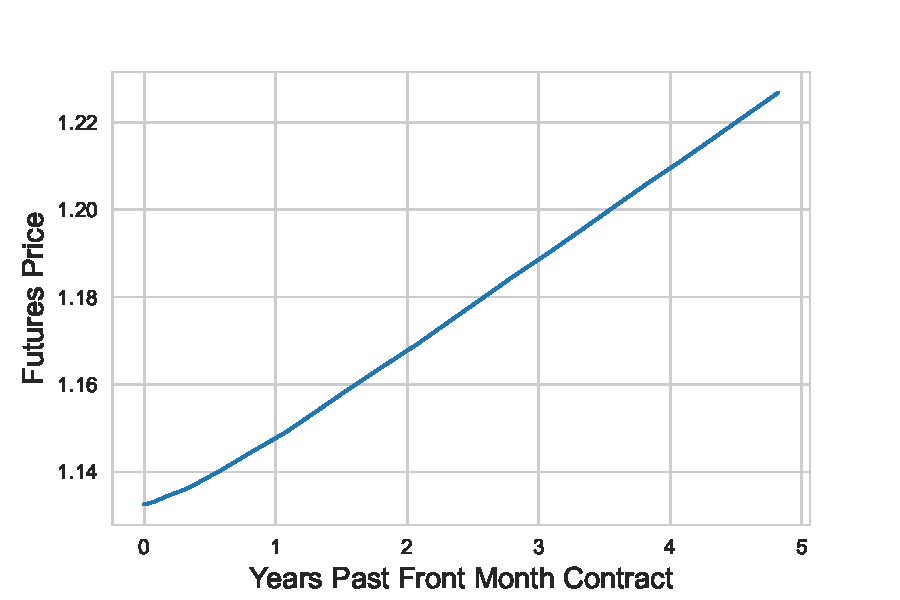
\includegraphics[scale=0.6]{Images/fig_euro.pdf}
    \end{center}
    Euro forward curve on 1-24-2022 (contango)
\end{frame}

\begin{frame}{Peso Forward Curve}
    \begin{center}
        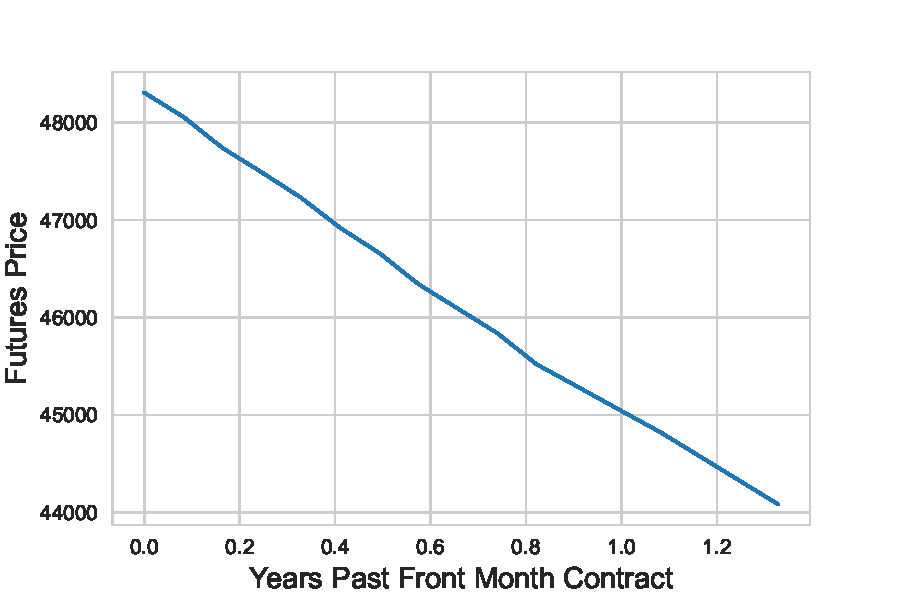
\includegraphics[scale=0.6]{Images/fig_peso.pdf}
    \end{center}
    Mexican peso forward curve on 1-24-2022 (backwardation)
\end{frame}

\begin{frame}{S\&P 500 Example}
    $S=$ spot index level, $F=$ futures price, $r=$ dollar interest rate, $y=$ dividend yield, meaning dividends on the basket of stock are $yS\,\D t$ per instant $\D t$.
    
    To own the basket in $T$ years, you need to buy $S\E^{-yT}$ dollars worth of stocks today.  If you borrow this, you will owe $S\E^{-yT}\E^{rT}$ in $T$ years, so $F=S\E^{(r-y)T}$ again.
\end{frame}

\begin{frame}{Stock Index Futures are in Backwardation}
 \begin{center}
        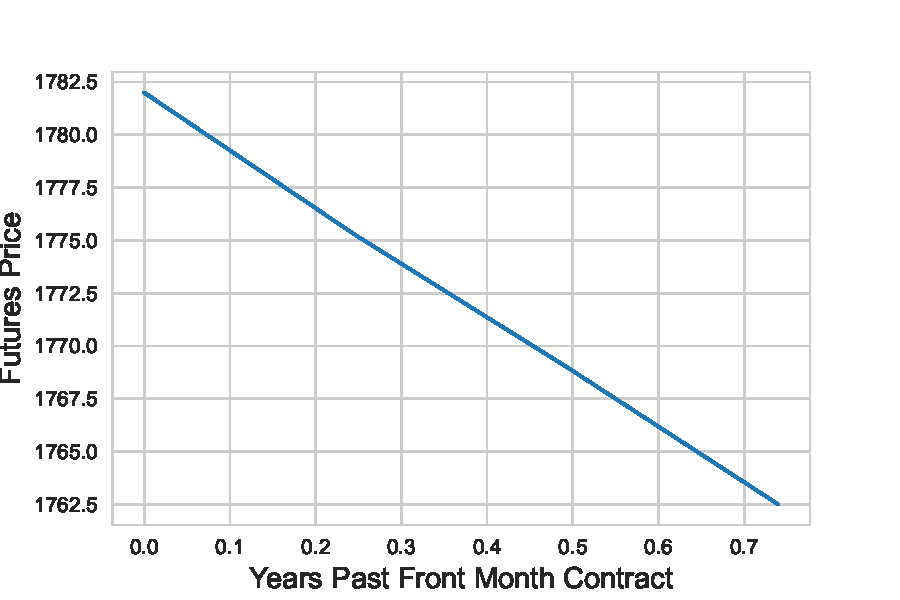
\includegraphics[scale=0.6]{Images/fig_sp500.pdf}
    \end{center}
    S\&P 500 forward curve on 1-24-2022
\end{frame}

\begin{frame}{Commodities}
    For commodities, the convenience yield is not so clear.
    
    If there is a spot shortage of a commodity, then it is `convenient' to own it today.  You can earn extra profits on it, like earning dividends on stocks or interest on currencies.
    
    However, storage costs are a `negative convenience' and can be large.
\end{frame}

\begin{frame}{Crude Oil Forward Curves}
    \begin{center}
        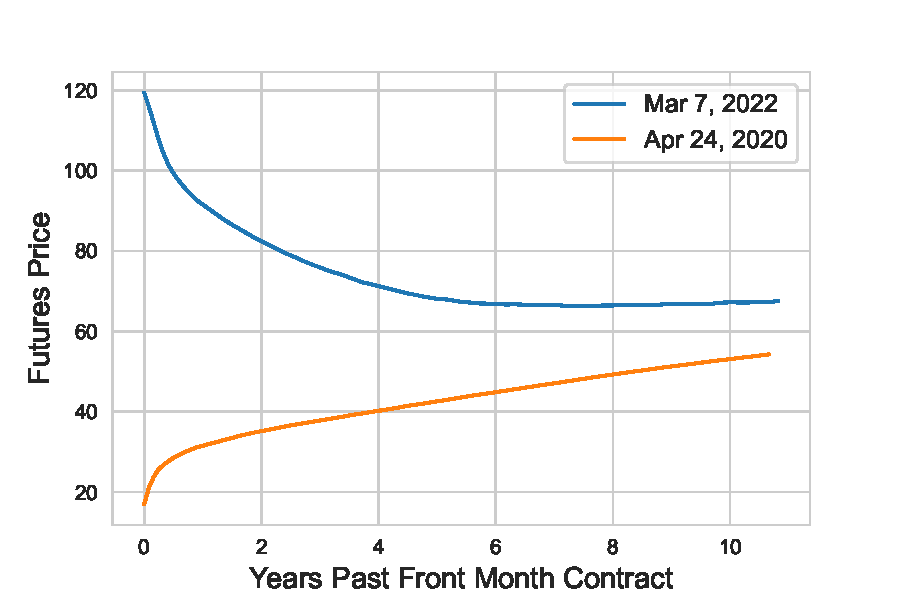
\includegraphics[scale=0.6]{Images/fig_crude.pdf}
    \end{center}
    Contango in 2020, backwardation in 2022
\end{frame}

\begin{frame}{Natural Gas}
    \begin{center}
        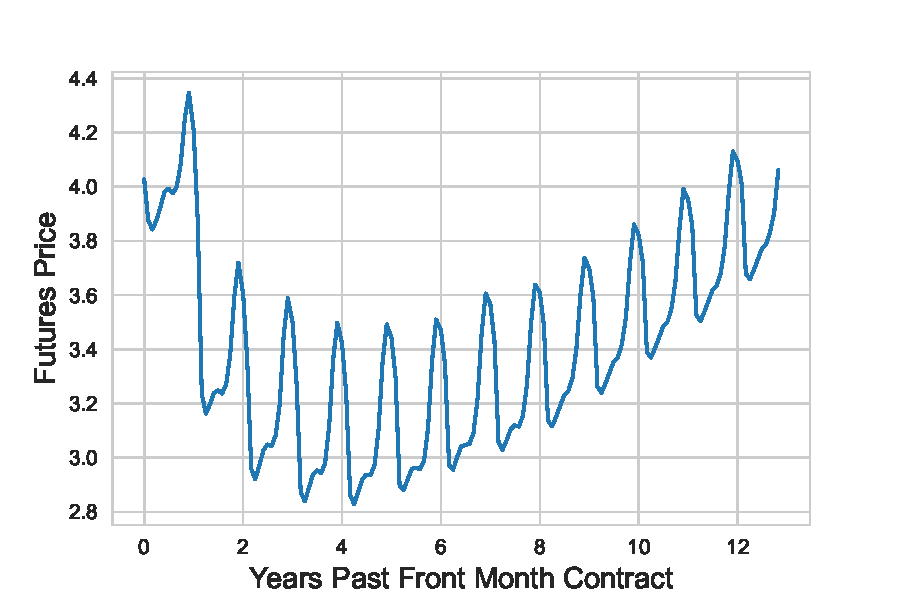
\includegraphics[scale=0.6]{Images/fig_ng.pdf}
    \end{center}
    Natural gas forward curve on 1-24-2022
\end{frame}

\begin{frame}{Gasoline}
    \begin{center}
        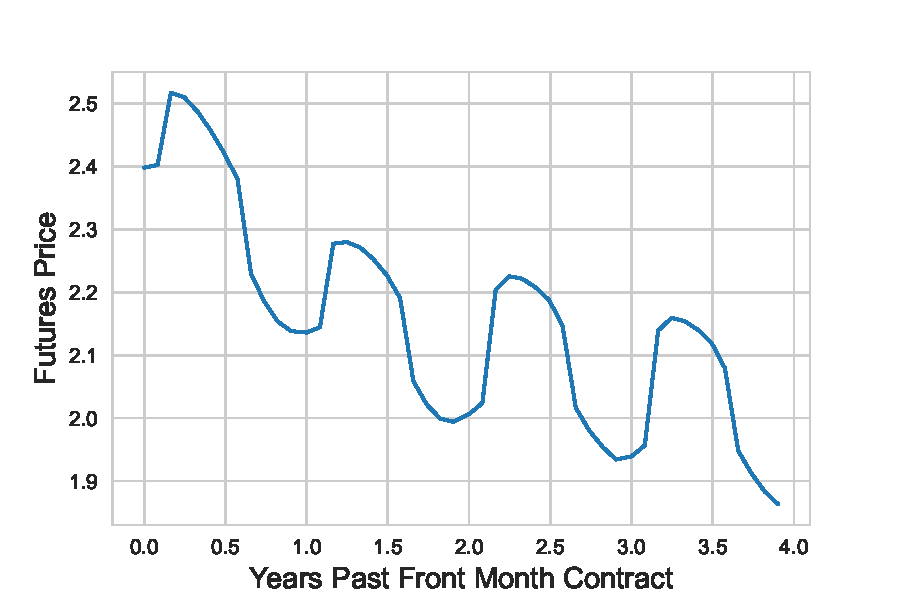
\includegraphics[scale=0.6]{Images/fig_rbob.pdf}
    \end{center}
    Gasoline
    forward curve on 1-24-2022
\end{frame}

\begin{frame}{SDFs}
    Let $M$ be an SDF process.  Suppose there is a security that pays \$1 for sure at date $T$.  This is called a zero-coupon bond or pure-discount bond.  Its price is 
    $\mye [M_T \times 1] = \mye[M_T]$.
    
    Define 
    $$r = \frac{-\log \mye[M_T]}{T}$$
    The number $r$ is the `annualized continuously compounded yield of the discount bond.'  The price of the discount bond is $\mye[M_T] = \E^{-rT}$.
    
    Let $X_T$ be the value of the `underlying asset' (currency, commodity, \ldots) at date $T$.  Suppose it doesn't pay any dividends or provide any convenience (like gold).  Ignore storage costs.  Then the price today is $S =\mye[M_TX_T]$.
\end{frame}

\begin{frame}{Forwards and SDFs}

    A forward contract (futures without marking to market) should have price $F$ such that it is a fair trade to pay $F$ for $X_T$ at date $T$.  This means $\mye[M_T(X_T-F)] = 0$.  Thus,
    $$0 = \mye[M_T(X_T-F)] = \mye[M_TX_T] -\mye[M_T]F = S - \E^{-rT}F$$
    
    So, $F = S\E^{rT}$.  If the asset pays a constant continuous convenience yield $y$ (like dividends or foreign interest), and $S$ is the price of 1 unit today, then the price today of getting 1 unit at $T$ is $S\E^{-yT}$, and we get $F = S\E^{(r-y)T}$ again.
    
    Futures are a little more complicated, especially if interest rates change over time.
    
    
\end{frame}

\begin{frame}{Expectations Hypothesis}
   A large empirical literature examines whether $F = \mye[X_T]$.  In other words, is the futures price the best forecast of the future spot price?
   
   If so, then when a market is in contango, the spot price is expected to rise.  When a market is in backwardation, the spot price is expected to fall.
   
   The expectations hypothesis fails empirically.  In currencies, this is called the `forward premium anomaly.'  When a currency market is in contango, the spot price generally falls a little rather than rising.  When it is in backwardation, the spot price generally rises a little.  This is equivalent to the success of the `currency carry trade.'  
   
   Currency carry trade: borrow in low interest rate countries and invest in high interest rate countries.
\end{frame}
\end{document}


\begin{frame

Cost of synthetic futures (for 1 yen):
$S\E^{rT}$ is the number of dollars you owe.  
The cost of buying spot and storing, including foregone interest on the cash investment, 
    
\end{frame}
\end{document}
    
    The settlement prices for subsequent days were
    \begin{align*}
        \text{Jan 3} \quad & \quad 51.72\\
        \text{Jan 6} \quad & \quad  51.81\\
        \text{Jan 7} \quad & \quad 52.13 \\
        \text{Jan 8} \quad & \quad 51.31
    \end{align*}
    Suppose you sold 1 contract on Jan 9 at \$51.50.  
\end{frame}
\begin{frame}[plain]
Here are the daily cash flows
\begin{align*}
       \text{Jan 2} \quad & \quad 51.80 & \quad \\
       \text{Jan 2} \quad & \quad 51.97 & \quad +170\\
        \text{Jan 3} \quad & \quad 51.72& \quad - 250\\
        \text{Jan 6} \quad & \quad  51.81& \quad + 90\\
        \text{Jan 7} \quad & \quad 52.13 & \quad +320\\
        \text{Jan 8} \quad & \quad 51.31& \quad - 820\\
        \text{Jan 9} \quad & \quad 51.50& \quad + 190
    \end{align*}
    The net is $-300 = \text{1,000} \times (51.50-51.80)$.
\end{frame}
    An agreement to transact at a later date.  One party will deliver and be paid.  The other party will accept delivery and will pay.
    
    Buyer (long) will accept delivery and will pay.  Seller (short) will deliver and be paid.
    
    Examples: energy (crude oil, natural gas, refined products), metals (gold, silver, \ldots), agricultural, currencies, financials (stock indexes, Treasury bonds, \ldots).
    
    Exchange traded.  Anyone can trade.  Usually buyer will later sell, and seller will later buy, so neither takes or makes delivery.
    
    Some traders are hedging.  Others are speculating.
\end{frame}
\end{document}